\chapter{Application mobile}
\label{chapter:app_mobile}
	\section{API REST}

		\subsection{Organisation des packages}

			L'organisation des packages se déroule comme suit :

			\begin{figure}[H]
				\centering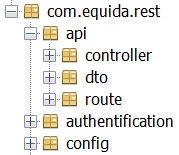
\includegraphics[width=0.23\textwidth, keepaspectratio]{res/package.png}
				\caption{Packages de l'api Rest}
			\end{figure}

			\begin{description}
				\item[api :]{Contient les fichiers de l'api}
				\begin{description}
					\item[controller :]{Contient tous les controleurs}
					\item[dto :]{Contient tous les Dto}
					\item[route :]{Contient toutes les routes}
				\end{description}
				\item[authentification :]{Contient la classe qui implémente BasicAuthenticationEntryPoint pour configurer Basic Authentification sur l'application}
				\item[config :]{Contient les classes de configuration et de sécurisation de l'application}
			\end{description}

		\subsection{Configuration de l'application}

			\subsubsection{application.properties}

			L'API Rest possède un fichier \textit{application.properties} qui permet de configurer certaines parties de l'application.

			\begin{figure}[H]
				\centering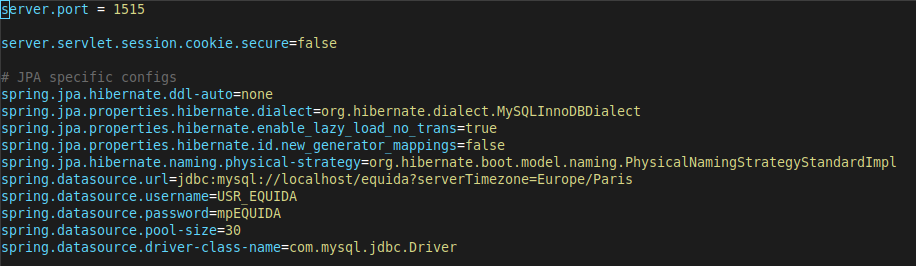
\includegraphics[width=0.85\textwidth, keepaspectratio]{res/application-properties.png}
				\caption{Configuration par application.properties}
			\end{figure}

			\noindent
			Ce fichier configure les informations relatives à l'application dans sa globalité, comme le port à utiliser, la configuration pour connexion avec la \bdd{} (nom utilisateur, mot de passe, ip, ...).

			\subsubsection{Configuration par le code}

			La configuration de Spring Security est directement faite dans le code source grace à l'utilisation de l'annotation @Configuration.

			\begin{figure}[H]
				\centering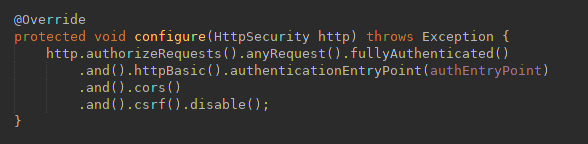
\includegraphics[width=0.75\textwidth, keepaspectratio]{res/config-httpsecurity.png}
				\caption{Configuration de Spring Security}
			\end{figure}

			\noindent
			Ici, on exige l'authentification sur toutes les requêtes faites à l'API. L'authentification doit être faite en utilisant \textit{Basic Authentification} (voir \nameref{subsec:basic_auth}). On y active les CORS et on désactive le csrf.

			\begin{figure}[H]
				\centering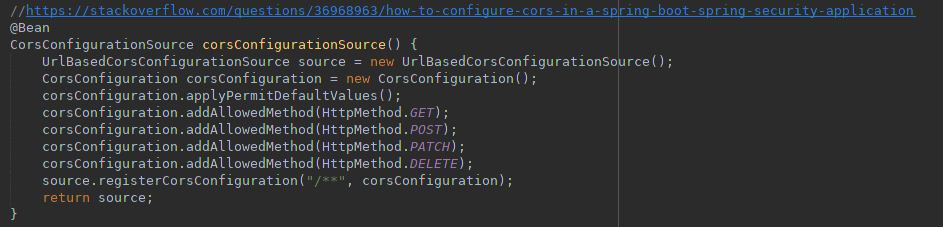
\includegraphics[width=0.75\textwidth, keepaspectratio]{res/config-cors.png}
				\caption{Configuration des requêtes CORS}
			\end{figure}

			\noindent
			Afin de permettre l'utilisation des requêtes DELETE et PATCH sur l'API, il a fallu changer la configuration des CORS. Le choix a été fait d'autoriser ces requêtes pour toutes les URL afin de simplifier la chose. Pour un code plus propre, il aurait fallu autoriser uniquement celles dont chaque URL avaient besoin.

			\begin{figure}[H]
				\centering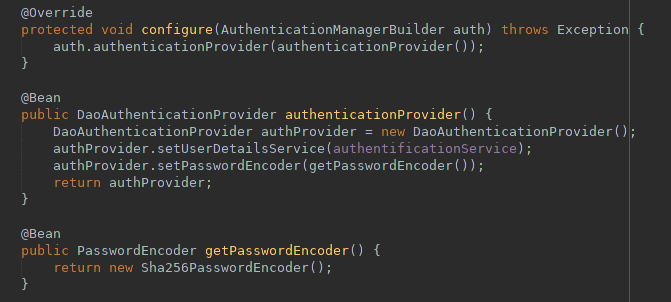
\includegraphics[width=0.75\textwidth, keepaspectratio]{res/config-authentification.png}
				\caption{Configuration de l'authentification}
			\end{figure}

			\noindent
			Enfin, comme pour WebApp, on définit le fonctionnement de l'authentification. Ainsi, vous pouvez retrouver les explications dans \nameref{sec:core_authentification}.

		\subsection{Système d'authentification sur l'API}
			\label{subsec:basic_auth}

			L'API utilisant \textit{Basic Authentification}, il est nécessaire de fournir à Spring Security une implémentation de ce modèle. C'est le rôle d'\textit{AuthenticationEntryPointImpl} dont voici le code :

			\begin{figure}[H]
				\centering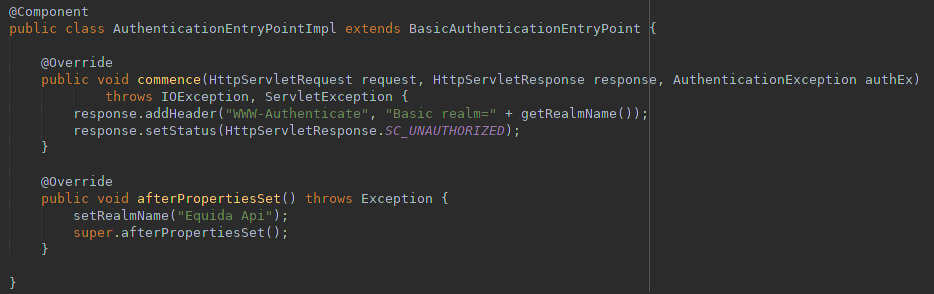
\includegraphics[width=0.75\textwidth, keepaspectratio]{res/AuthenticationEntryPointImpl.png}
				\caption{Code d'AuthenticationEntryPointImpl}
			\end{figure}

			\noindent
			Le code reste extrêmement simple ici car Spring Security nous offre une couche d'abstraction pour l'implémentation du modèle. Ainsi, le seul élément que l'on définit est le realm.

		\subsection{Exemple Route}

			L'interface \textit{IRoute} décrit la méthode qui doit être implémentée par les classes filles.\newline
			Ainsi chaque fichier route contiendra une méthode \textit{getUri()} qui retournera l'URL à utiliser dans la page concernée (pour la route correspondante).

			\noindent
			Par exemple, pour \textit{LotsApiRoute}, qui est donc la route principale de l'api pour la gestion des lots selon notre nomenclature, l'URL renvoyée est \textit{/api/lots}.

			\begin{figure}[H]
				\centering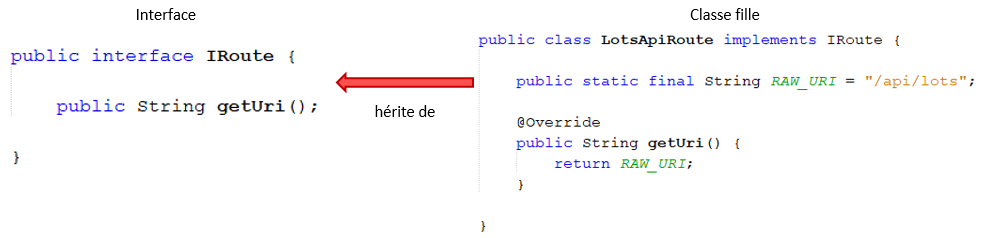
\includegraphics[width=0.80\textwidth, keepaspectratio]{res/IRoute.png}
				\caption{Interface IRoute et exemple avec LotsApiRoute}
			\end{figure}

		\newpage
		\subsection{Les Dto}

			\subsubsection{L'interface IDto}

				Afin d'alléger les requêtes SQL à la \bdd{} et la sortie en JSON des classes métiers, le choix à été fait d'utiliser les DTO. Aucun lien vers un autre objet n'est fait, seul son ID est laissé et il faudra ensuite utiliser l'URL adéquate afin de récupérer les informations si celles-ci nous intéressent.

				\noindent
				Pour uniformiser nos DTO, une interface IDto a été faite.

				\begin{figure}[H]
					\centering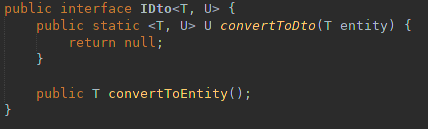
\includegraphics[width=0.75\textwidth, keepaspectratio]{res/idto.png}
					\caption{Code de l'interface IDto}
				\end{figure}

				\noindent
				Celle ci se base donc sur une généricité double, T étant notre classe métier provenant du package \textit{com.equida.common.bdd.entity} et U étant la classe DTO correspondante. Cette interface définit 2 méthodes, \textit{<T, U> U convertToDto(T entity)} permettant de convertir une instance de nos classes Métier en un DTO et \textit{T convertToEntity()} qui permet de convertir notre DTO en une instance de nos classes Métier.

			\subsubsection{Exemple de Dto}

			\begin{figure}[H]
				\centering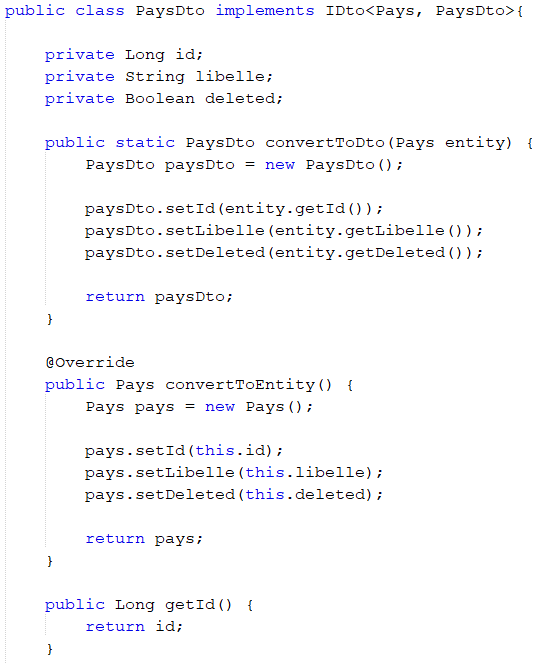
\includegraphics[width=0.35\textwidth, keepaspectratio]{res/paysDto.png}
				\caption{Exemple code de PaysDto}
			\end{figure}

		\newpage
		\subsection{Exemple Controller}

			Les différents contrôleurs sont des classes précédées de l'annotation @RestController. \newline
			Les contrôleurs contiennent différentes méthodes associées aux méthodes GET, POST, PATCH et DELETE ainsi qu'a une route. Enfin elles utilisent les services pour intéragir avec la \bdd{}. On y définit aussi les différentes autorisations avec l'annotation @PreAuthorize afin de savoir qui peut accéder à la page, et donc, executer la méthode.

			\noindent
			Par exemple, pour \textit{LotDetailsRestController}, on implémente la méthode \textit{getLot}, liée à la route \textit{LotDetailsApiRoute.RAW\_URI}, qui prend en paramètre l'id du lot concerné. Elle va retourner (grâce à la méthode \textit{getById} de \textit{LotService}) le lot correspondant sous la forme d'un \textit{LotDto}.

			\begin{figure}[H]
				\centering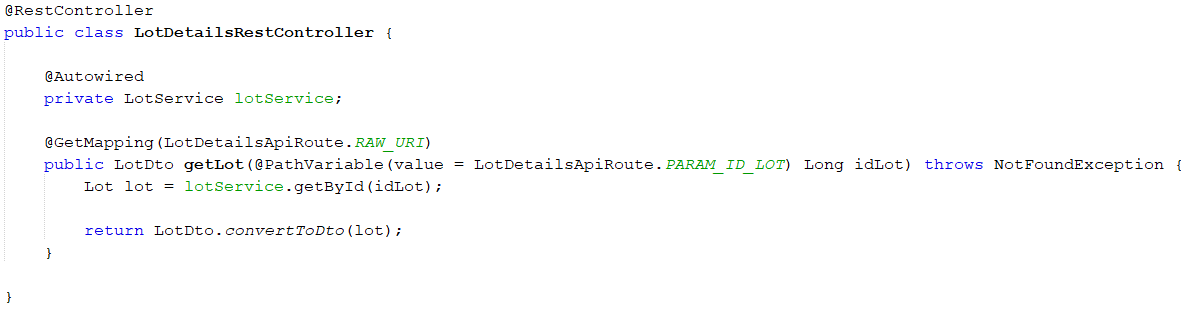
\includegraphics[width=0.80\textwidth, keepaspectratio]{res/lotsController.png}
				\caption{Exemple d'un contrôleur avec LotDetailsRestController}
			\end{figure}


	\section{Ionic}

		\subsection{Organisation des packages}

			L'organisation des packages se déroule comme suit :

			\begin{figure}[H]
				\centering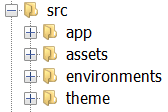
\includegraphics[width=0.33\textwidth, keepaspectratio]{res/ionicPackage.png}
				\caption{Packages de ionic}
			\end{figure}

			\begin{description}
				\item[app :]{Contient les fichiers de l'applicaton}
				\item[assets :]{Contient les images de l'applications}
				\item[environments :]{Contient les différents "mode de fonctionnement" de l'application. On aura par exemple un environnement de développement (utilisé par défaut) ainsi qu'un autre pour faire fonctionner l'application en mode production. On pourra ainsi affiner le niveau de debug et de log pour voir, ou non, plus d'erreur et intégrer des outils pour simplifier le débugguage de l'application.}
				\item[theme :]{Contient le fichier variables.scss qui définit les couleurs utilisées par ionic}
			\end{description}

		\subsection{Les pages}

			Les différentes pages générées (via la commande \textit{ionic g}) suivent la même nomenclature : elles sont placées dans un dossier du nom de l'entité concernée suivit d'un verbe (souvent : lister, ajouter, consulter, modifier). \newline

			\begin{figure}[H]
				\centering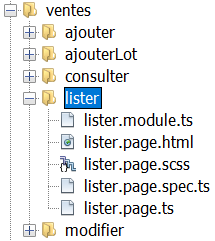
\includegraphics[width=0.33\textwidth, keepaspectratio]{res/ionicListerVentes.png}
				\caption{Résultat de la commande \textit{ionic g} avec un nom de page correspondant à lister dans le dossier ventes}
			\end{figure}

			\noindent
			Dans chaque sous-dossier (un sous-dossier pour lister, un pour ajouter, ...) crée par la commande ionic, on retrouvera les mêmes types de fichiers.\newline

			\begin{description}
				\item[x.module.ts :]{Exporte notre module pour être utilisable par ionic}
				\item[x.page.html :]{Contient le code HTML de la page ainsi que les composants ionic}
				\item[x.page.scss :]{Permet de modifier le style de la page}
				\item[x.page.spec.ts :]{Permet d'effectuer des tests unitaires}
				\item[x.page.ts :]{Contient toutes les méthodes à éxécuter ainsi que l'initialisation de la page}
			\end{description}

			\noindent
			On ne travaillera que sur les fichiers x.page.ts, x.page.html.

			\subsubsection{Lister}

					La page \textit{lister.page.html}, contient donc un header avec le titre de la page, ainsi qu'un content avec la liste et une boucle permettant l'affichage des ventes (\textit{*ngFor="let v of ventes"}) et la gestion d'un clic sur une vente (\textit{routerLink="/ventes/{{v.id}}"}) qui renvoie donc sur la page de la vente en question. \newline
					On retrouve aussi un test sur le role de l'utilisateur (\textit{*ngIf="role == 'ADMIN'"}), si l'utilisateur a un role 'ADMIN' alors il verra un bouton flottant d'ajout. Ce bouton le renverra vers la page d'ajout d'une vente. \newline
					Pour finir, on affiche plus de ventes sur la page lors d'un scroll de l'utilisateur si celui ci atteint le bas de la page.

					\begin{figure}[H]
						\centering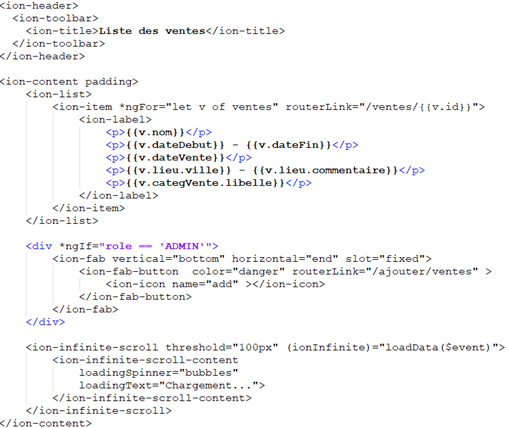
\includegraphics[width=0.9\textwidth, keepaspectratio]{res/lister.png}
						\caption{Code de /ventes/lister/lister.page.html}
					\end{figure}

					La page \textit{lister.page.ts}, contient le constructeur, l'initialisation des variables, l'initialisation de la page avec la méthode \textit{ngOnInit} qui appelle notamment la méthode \textit{getVentes}. Cette méthode appelle la méthode \textit{loadVentes} qui chargera donc les ventes, pour peu qu'il en reste à récupérer (et qui récupèrera le lieu et la catégorie de vente, par leur id respectif, afin de les afficher).

					\begin{figure}[H]
						\centering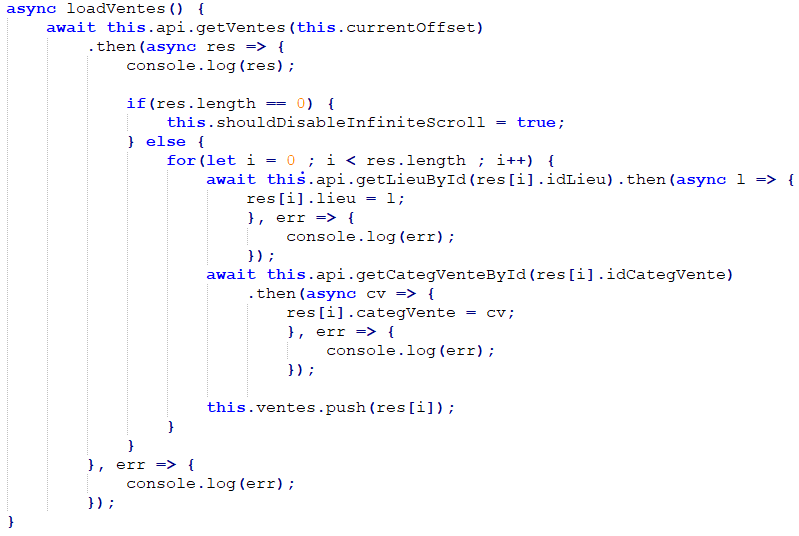
\includegraphics[width=0.9\textwidth, keepaspectratio]{res/listerTs.png}
						\caption{Code méthode loadVentes de /ventes/lister/lister.page.ts}
					\end{figure}

					\begin{figure}[H]
						\centering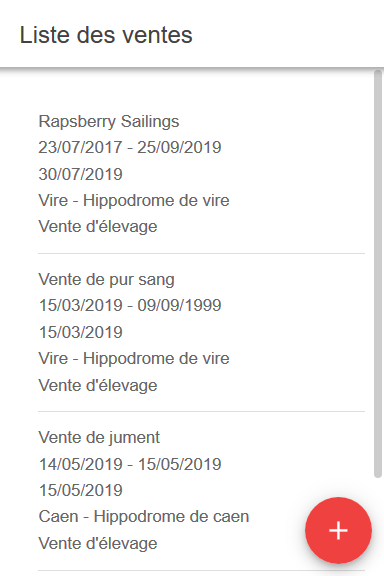
\includegraphics[width=0.33\textwidth, keepaspectratio]{res/listerVentes.png}
						\caption{Résultat de la page lister les ventes}
					\end{figure}

			\subsubsection{Consulter}

			La page \textit{consulter.page.html}, contient donc un header avec le titre de la page ; ainsi qu'un content avec un composant ionic card (purement visuel) dans lequel on retrouve des items correspondant aux différents champs d'une vente.\newline
			Puisque c'est une page de consultation, les champs affichent les valeurs contenues dans la base de données.\newline
			On trouve, là-aussi des boutons. Un pour proposer un cheval, seulement disponible pour un utilisateur classique ainsi qu'un pour supprimer, présent seulement si l'utilisateur connecté est un administrateur. \newline
			Sur le même principe, on a aussi la liste des lots en vente (que l'on affiche pas ci-dessous dans le code mais qui est présent dans le fichier).

			\begin{figure}[H]
				\centering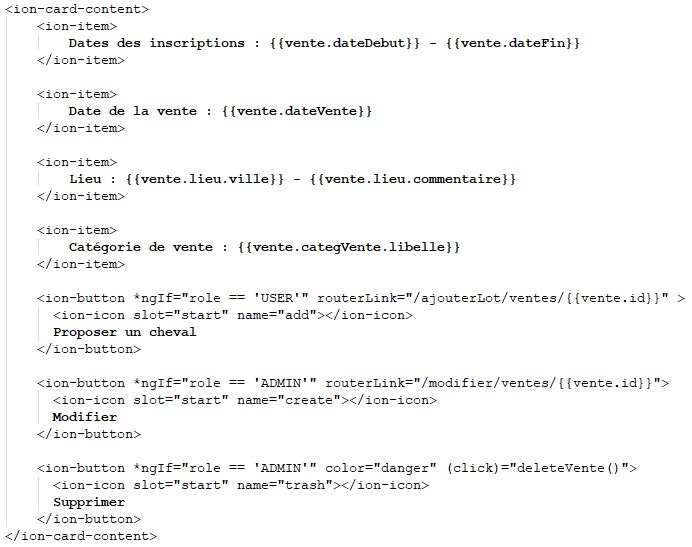
\includegraphics[width=0.9\textwidth, keepaspectratio]{res/consulter.png}
				\caption{Extrait du code de /ventes/consulter/consulter.page.html}
			\end{figure}

			La page \textit{consulter.page.ts}, contient le constructeur, l'initialisation des variables, l'initialisation de la page avec la méthode ngOnInit qui appelle notamment les méthodes \textit{getVenteById} et \textit{getLotsByIdVente}.\newline
			La méthode \textit{getVenteById} se charge donc de récupérer la vente par l'id passé en paramètre de la route. Afin d'afficher le lieu et la catégorie de vente, elle utilise aussi les méthodes \textit{getLieuById} et \textit{getCategVenteById} de l'api qui renvoient le bon nom, libellé en fonction de l'id fourni par la vente affichée.\newline
			On trouve aussi la méthode \textit{deleteVente} appelée lors du clic sur le bouton supprimer. La vente dont l'id est passé en paramètre sera supprimée et l'utilisateur sera redirigé vers la page des ventes.

			\begin{figure}[H]
				\centering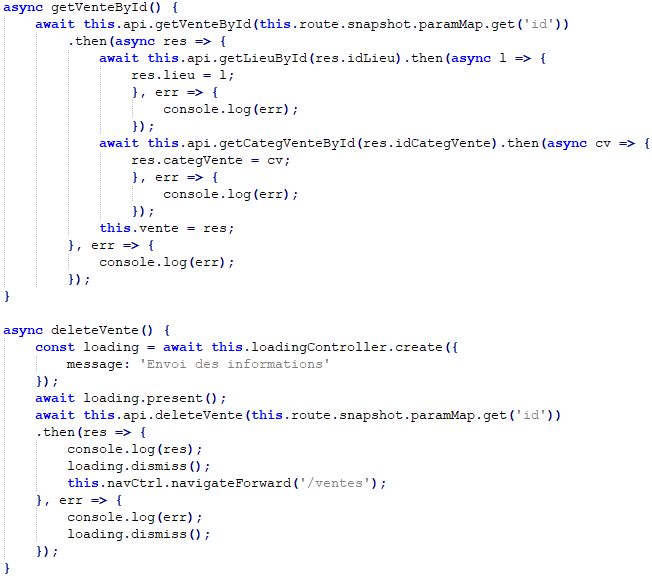
\includegraphics[width=0.9\textwidth, keepaspectratio]{res/consulterTs.png}
				\caption{Extrait du code de /ventes/consulter/consulter.page.ts}
			\end{figure}

			\begin{figure}[H]
				\centering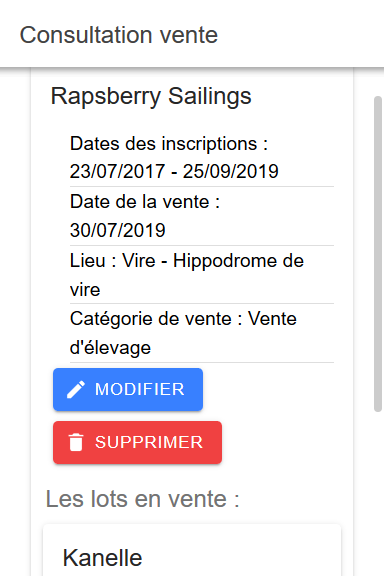
\includegraphics[width=0.33\textwidth, keepaspectratio]{res/consulterVente.png}
				\caption{Résultat de la page de consultation d'une vente}
			\end{figure}

			\subsubsection{Ajouter}

			La page \textit{ajouter.page.html}, contient donc un header avec le titre de la page ; ainsi qu'un content avec les différents items et input. \newline
			Dans les input et les select, on retrouve \textit{[(ngModel="nomChamp")]} qui fera donc le lien entre les données saisies dans ce champ et les variables associées.\newline
			On a aussi un bouton qui lorsqu'il est cliqué, appelle la méthode \textit{addVente}.

			\begin{figure}[H]
				\centering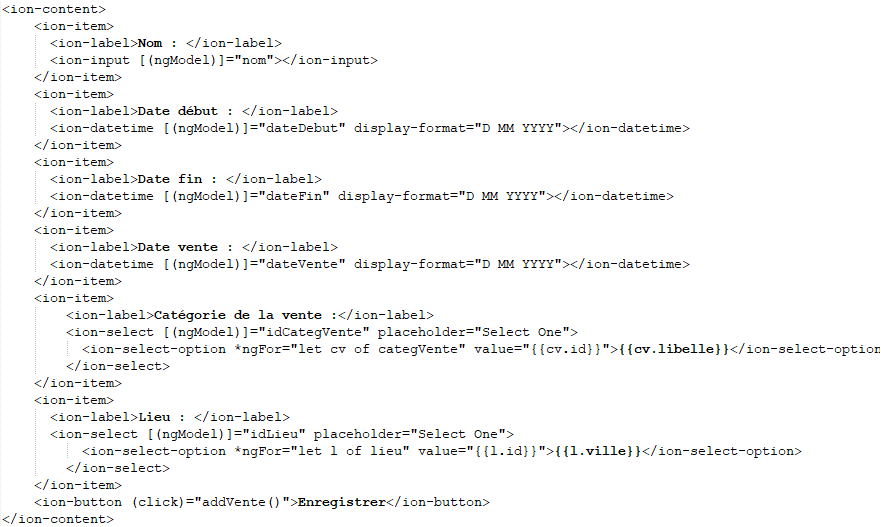
\includegraphics[width=0.9\textwidth, keepaspectratio]{res/ajouter.png}
				\caption{Code de /ventes/ajouter/ajouter.page.html}
			\end{figure}

			La page \textit{ajouter.page.ts}, contient le constructeur, l'initialisation des variables, l'initialisation de la page avec la méthode \textit{ngOnInit} qui appelle notamment les méthodes getCategVente et getLieux de l'api.\newline
			La méthode addVente se chargera donc de créer la vente grâce aux paramètres passés dans la méthode de l'api.

			\begin{figure}[H]
				\centering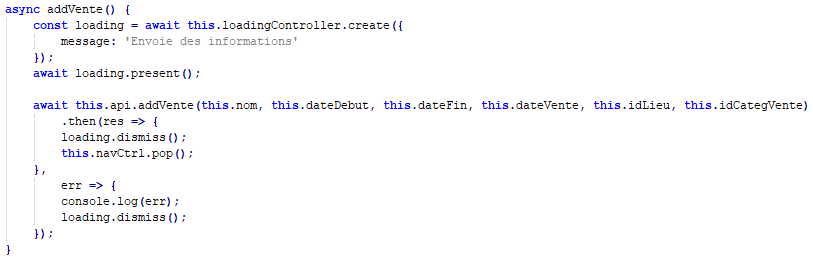
\includegraphics[width=0.9\textwidth, keepaspectratio]{res/ajouterTs.png}
				\caption{Extrait du code de /ventes/ajouter/ajouter.page.ts}
			\end{figure}

			\begin{figure}[H]
				\centering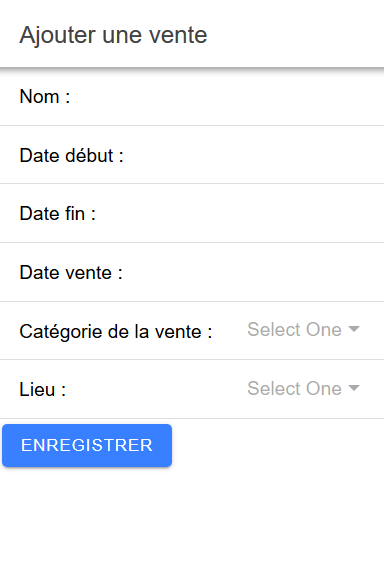
\includegraphics[width=0.33\textwidth, keepaspectratio]{res/ajouterVente.png}
				\caption{Résultat de la page d'ajout d'une vente}
			\end{figure}

			\subsubsection{Modifier}

			La page \textit{modifier.page.html}, est sensiblement la même que \textit{ajouter.page.ts}. A la différence que le bouton, lorsqu'il est cliqué, appelle la méthode \textit{updateVente}.

			La page \textit{modifier.page.ts}, contient le constructeur, l'initialisation des variables, l'initialisation de la page avec la méthode \textit{ngOnInit} qui récupère les valeurs de la vente à modifier.\newline
			La méthode \textit{updateVente} se chargera donc de modifier la vente grâce aux paramètres passés dans la méthode de l'api.

			\begin{figure}[H]
				\centering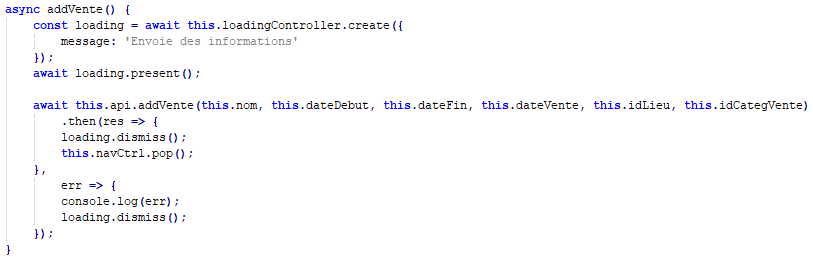
\includegraphics[width=0.9\textwidth, keepaspectratio]{res/ajouterTs.png}
				\caption{Extrait du code de /ventes/modifier/modifier.page.ts}
			\end{figure}

			\begin{figure}[H]
				\centering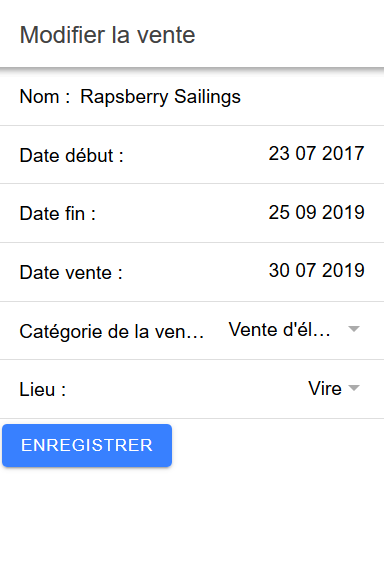
\includegraphics[width=0.33\textwidth, keepaspectratio]{res/modifierVente.png}
				\caption{Résultat de la page de modification d'une vente}
			\end{figure}

		\subsection{Rest Api}

			Pour faciliter l'éxécution des différentes requêtes à l'API la classe \textit{rest-api.service} a été conçue.

			\subsubsection{Authentification à l'Api}

				\begin{figure}[H]
					\centering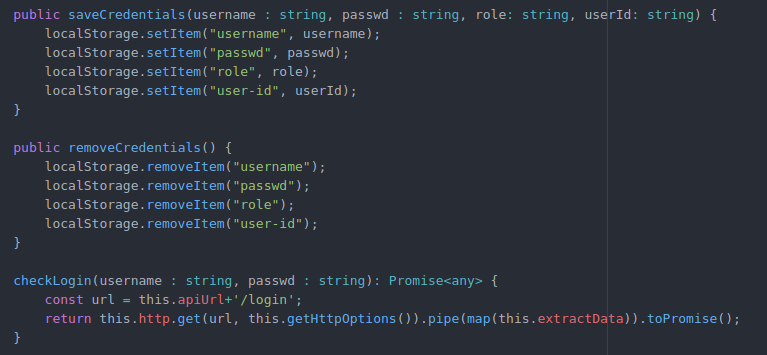
\includegraphics[width=0.75\textwidth, keepaspectratio]{res/ionic-rest-auth.png}
					\caption{Code de la classe RestApiService}
				\end{figure}

				\noindent
				Ici, \textit{saveCredentials} permet d'enregistrer les informations relatives à l'authentification du client dans le local storage. Il existe \textit{removeCredentials} qui elle, à l'inverse de \textit{saveCredentials}, supprime les informations relatives à l'utilisateur connecté. On a ainsi 2 méthodes qui permettent de gérer facilement la connexion et la déconnexion d'un utlisateur.

				\noindent
				La méthode \textit{checkLogin} permet d'appeller \textit{/api/login} et d'obtenir les informations relatives à l'utilisateur si les informations fournies sont correctes.

				\begin{figure}[H]
					\centering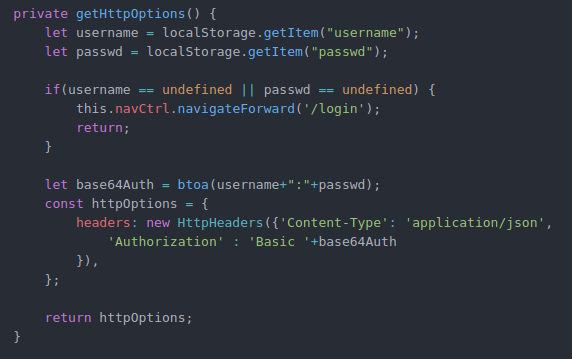
\includegraphics[width=0.70\textwidth, keepaspectratio]{res/ionic-rest-httpoptions.png}
					\caption{Code de la classe RestApiService}
				\end{figure}

				\noindent
				Ces informations sont ensuite réutilisées pour permettre l'authentification à l'API. Pour cela, la méthode \textit{getHttpOptions} permet d'obtenir l'entête à founir pour chaque appel à l'API. Dans le cas où le mot de passe ou le login est null, on redirige l'utilisateur vers la page de connexion.

			\subsubsection{Execution des différentes méthodes}

				Les appels à l'API utilisant les méthode HTTP GET, POST, PATCH et DELETE, une méthode existe, dans la classe \textit{rest-api.service}, pour chacune de ces méthodes HTTP. Voici un exemple avec la méthode HTTP GET.

				\begin{figure}[H]
					\centering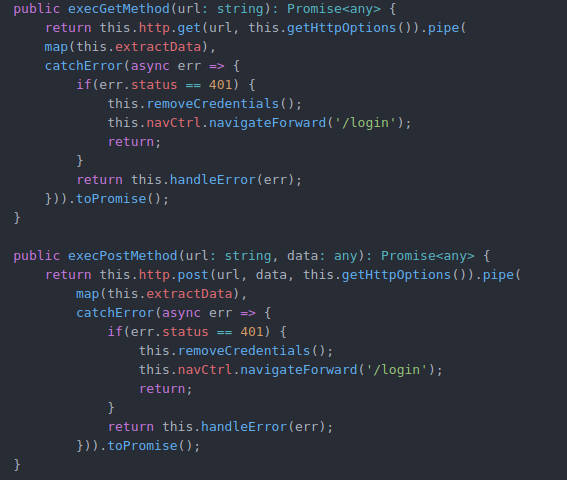
\includegraphics[width=0.70\textwidth, keepaspectratio]{res/ionic-rest-execmethod.png}
					\caption{Code de la méthode HHTP GET}
				\end{figure}

				\noindent
				On effectue, ici, l'appel à l'url fourni en paramètre tout en récupérant les entêtes nécessaires pour l'authentification. Selon si l'appel a réussi ou non, on retourne le résultat ou on appelle \textit{handleError} afin de générer un message d'erreur ainsi qu'une exception. Il est important de vérifier si le code d'erreur est 401 car si c'est le cas, l'utilisateur est, ou désactivé, ou alors a son mot de passe de changé. Si tel est le cas, on le déconnecte et on le redirige vers la page de connexion.

				\noindent
				Les autres méthodes ne changent pas tellement si ce n'est que pour POST et PATCH on fournit en plus un objet "data" qui correspond aux informations à fournir à l'API mais aussi le nom des méthodes appellées sur l'objet HTTP CHANGE.

				\begin{figure}[H]
					\centering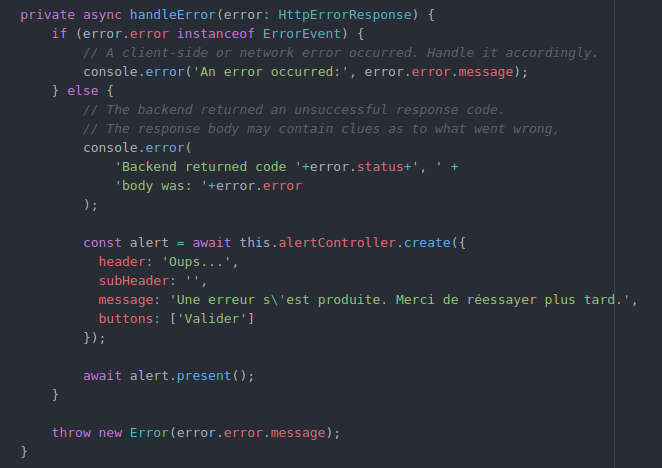
\includegraphics[width=0.75\textwidth, keepaspectratio]{res/ionic-rest-error.png}
					\caption{Code de la methode handleError}
				\end{figure}

				\noindent
				La méthode \textit{handleError} affiche les informations à propos de l'erreur dans la console du navigateur et se charge également d'afficher une boite de dialogue expliquant qu'une erreur est survenue. Dans le cadre du développement, cela permet également de rappeler que plus d'informations sont disponibles dans la console.

			\newpage
			\subsubsection{Exemples}

			Ainsi, l'appel aux différents endpoints de l'API tient en quelques lignes et se retrouve extrêmement simpifié comme on peut le voir sur les méthodes suivantes :

				\begin{figure}[H]
					\centering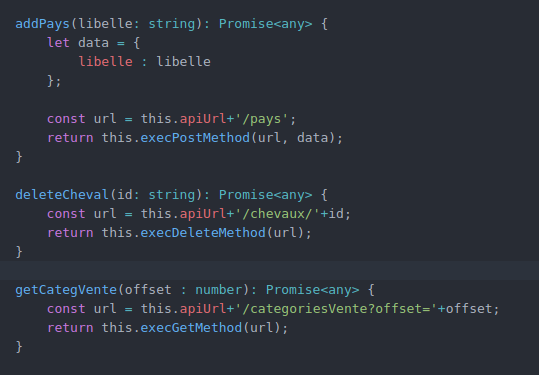
\includegraphics[width=0.75\textwidth, keepaspectratio]{res/ionic-rest-add-delete-get.png}
					\caption{Code des appels}
				\end{figure}

			\noindent
			Le fait de retourner une instance de \textit{Promise} permet d'utiliser \textit{await} sur la méthode et donc d'attendre la réponse de l'API avant de continuer l'éxécution du code.

		\subsection{Problèmes connus}

			Cette application mobile comporte des erreurs sur lesquelles nous n'avons pas pu, su intervenir.

			\noindent
			En effet, après un ajout ou une modification (quelque soit l'entité concernée), lorsque l'utilisateur est redirigé vers la page principale (celle qui liste), les informations ne sont pas mises à jour car la page n'est pas actualisée. \newline
			Afin de palier à cette erreur, il est nécessaire d'actualiser "manuellement" la page.

			\noindent
			Actuellement, en cas d'erreur sur les formulaires, une boite de dialogue avec le message "oups, une erreur est survenue" s'affiche. A terme, il faudrait afficher un message sur l'écran expliquant le champs sur lequel l'erreur est survenue ainsi que la raison de celle ci. Cela est actuellement impossible à faire car il faut restructurer la façon donc \textit{rest-api.service} fonctionne afin d'y permettre, d'une part, une meilleure gestion des erreurs, d'autre part le fait de ne pas afficher la boite de dialogue systématiquement dans le cas où l'API retourne un code d'erreur.
